\documentclass[a4paper]{article}

% ===== Packages =====
\usepackage[T1]{fontenc}        % Font encoding
\usepackage{lmodern}
\usepackage{algorithm}
\usepackage{subcaption}

% Modern font
\usepackage[a4paper,margin=0.8in]{geometry} % Page layout: 1in margin
\usepackage[fleqn]{amsmath}     % Math symbols, left-aligned equations
\setlength{\mathindent}{0pt}    % No indent for fleqn
\usepackage{amssymb}            % Extra math symbols
\usepackage{booktabs}           % Better tables
\usepackage{graphicx}           % Include graphics
\usepackage{setspace}           % Adjust line spacing
\usepackage{titling}            % Customize title format
\usepackage{float}              % [H] for figure placement
\usepackage{color}              % For colored text
\usepackage{booktabs}           % For better tables
\usepackage[colorlinks=true, linkcolor=blue, citecolor=blue, urlcolor=blue]{hyperref}
\usepackage{algorithm}
\usepackage{algorithmic}
\renewcommand{\thealgorithm}{\arabic{algorithm}} % Numerazione autonoma

\newcommand{\todo}[1]{\textcolor{red}{\textbf{TODO:} #1}}

% ===== Line spacing =====
\setstretch{0.9}                % 0.9× spacing; regola a piacere

% ===== Title formatting =====
\pretitle{%
  \begin{center}\bfseries\Large
  }
  \posttitle{%
  \end{center}\vspace{-1em}
}
\preauthor{%
  \begin{center}\small
  }
  \postauthor{%
  \end{center}\vspace{-1em}
}
\predate{}  % no date before
\postdate{} % no date after

% ===== Metadata =====
\title{Report HW4}
\author{%
  \ifdefined\anonymous%
  Anonymous Submission
  \else
  \begin{tabular}{cc}
    Simone De Carli & Damiano Salvaterra \\
    {\small\texttt{simone.decarli@studenti.unitn.it}} &
    {\small\texttt{damiano.salvaterra@studenti.unitn.it}}
  \end{tabular}
  \fi
}
\date{}  % leave date blank

\begin{document}

\maketitle

\section*{Exercise 1}

We implemented a MM1 queue simulator that consits of three main components:
\begin{itemize}
    \setlength\itemsep{0.01em}
  \item \textbf{Event}: represents the arrival or departure at a certain time;
  \item \textbf{Scheduler}: given a drawn event, it inserts in the min-heap of the future events;
  \item \textbf{MM1}: represents the internal queue system allowing to enqueue and dequeue packets, storing the current number of packets in the queue and if the server is busy or not;
  \item \textbf{Simulator}: act as a controller, it initializes the system and orchestrates the previous components. It also logs to a file the states of the system at each event. Terminates the simulation when a stopping condition is met (time limit, number of events, etc.).
\end{itemize}

\subsection*{Part 1: Show how the number of packets in the system changes over time}

We ran a simulation with $\lambda = 1$ and $\mu = 1.5$ stopping after 1000 time units. Figure~\ref{fig:e1p1-pis} shows the number of packets in the system over time and, in yellow, the moving average of the number of packets in the system that after a warm-up period visually converges to the theoretical value of $\frac{\rho}{1 - \rho} = 2$.
The server utilization is shown in Figure~\ref{fig:e1p1-util}, where the moving average converges to a slightly lower value (0.6) than the theoretical value of $\rho = \frac{\lambda}{\mu} = \frac{2}{3} \approx 0.67$.

\begin{figure}[htbp]
  \centering
  \begin{subfigure}[t]{0.4\textwidth}
    \centering
    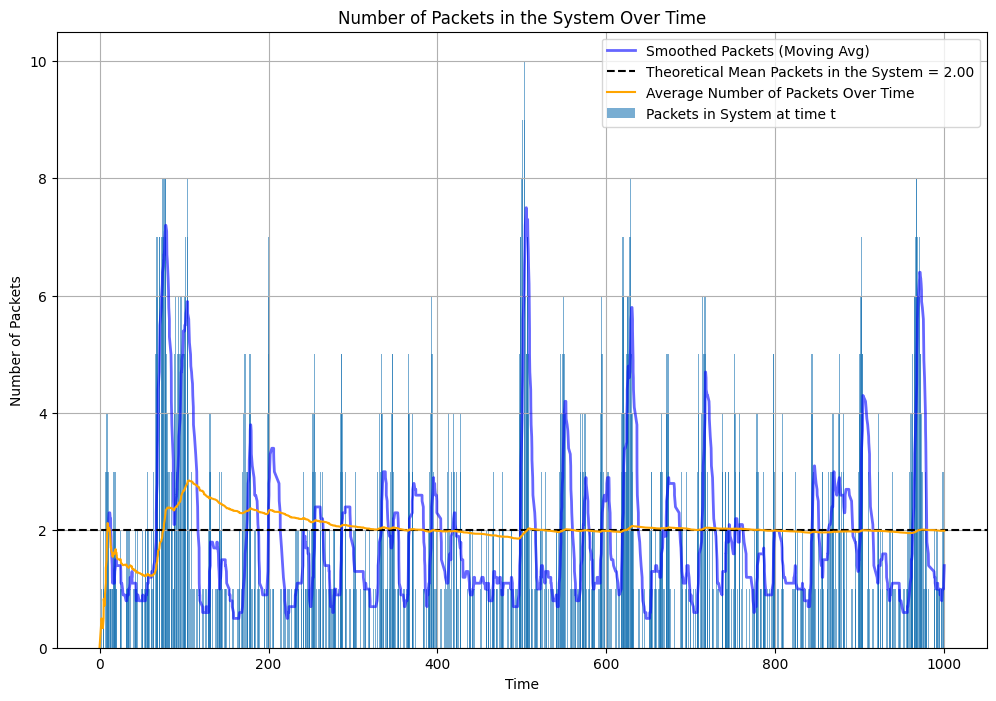
\includegraphics[width=\textwidth]{images/ex1_p1_pis_ot.png}
    \caption{
      Number of packets in the system over time.
    }\label{fig:e1p1-pis}
  \end{subfigure}
  \hfill
  \begin{subfigure}[t]{0.4\textwidth}
    \centering
    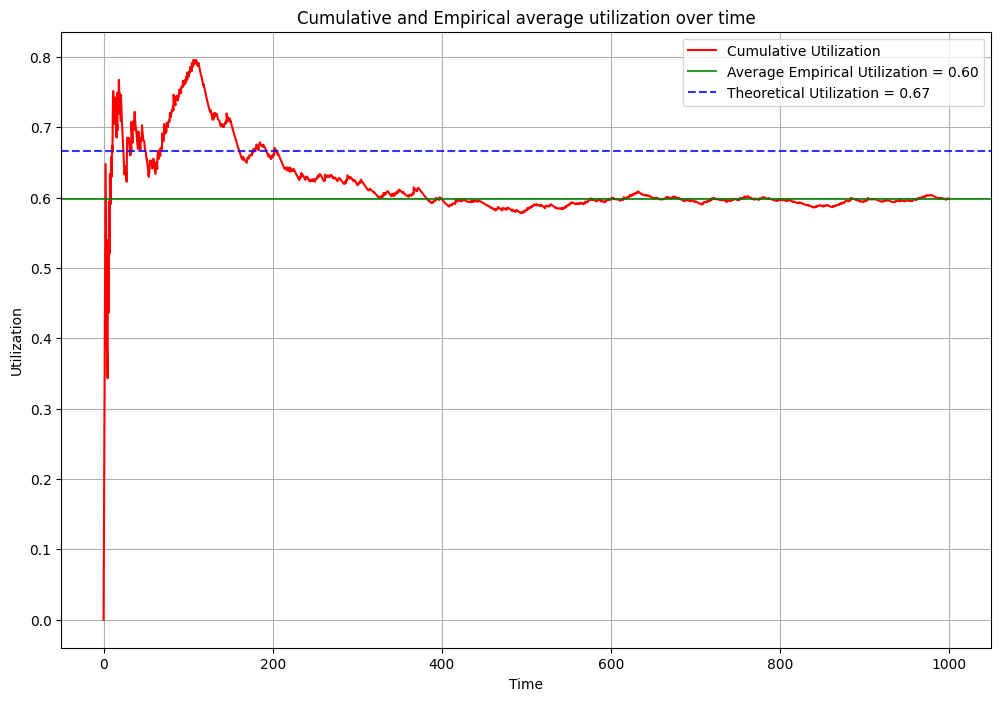
\includegraphics[width=\textwidth]{images/ex1_p1_util_ot.png}
    \caption{
      Server utilization over time.
    }\label{fig:e1p1-util}
  \end{subfigure}
  \caption{
    The number of packets in the system and the server utilization over time.
    The empirical data tends to converge to the theoretical values for $\lambda = 1$ and $\mu = 1.5$.
  }\label{fig:e1p1}
\end{figure}

\subsection*{Part 2: Test the simulator with different values of $\lambda$ and $\mu$}

For all combinations of $\lambda \in \{0.5, 1, 1.5\}$ and $\mu \in \{1, 1.5, 2\}$, stopping after 1000 time units.
For each combination, we ran 25 independent replications and computed the average empirical utilization.

Figure~\ref{fig:e1p2-util} shows the average empirical utilization over time (averaged through the 25 replications) for each combination of $\lambda$ and $\mu$.
It is possible to see that only blue lines (where $\lambda < \mu$) converge to a stable value, while the other two (red and yellow) saturate to 1, indicating that the system is unstable.

\begin{figure}[htbp]
  \centering
  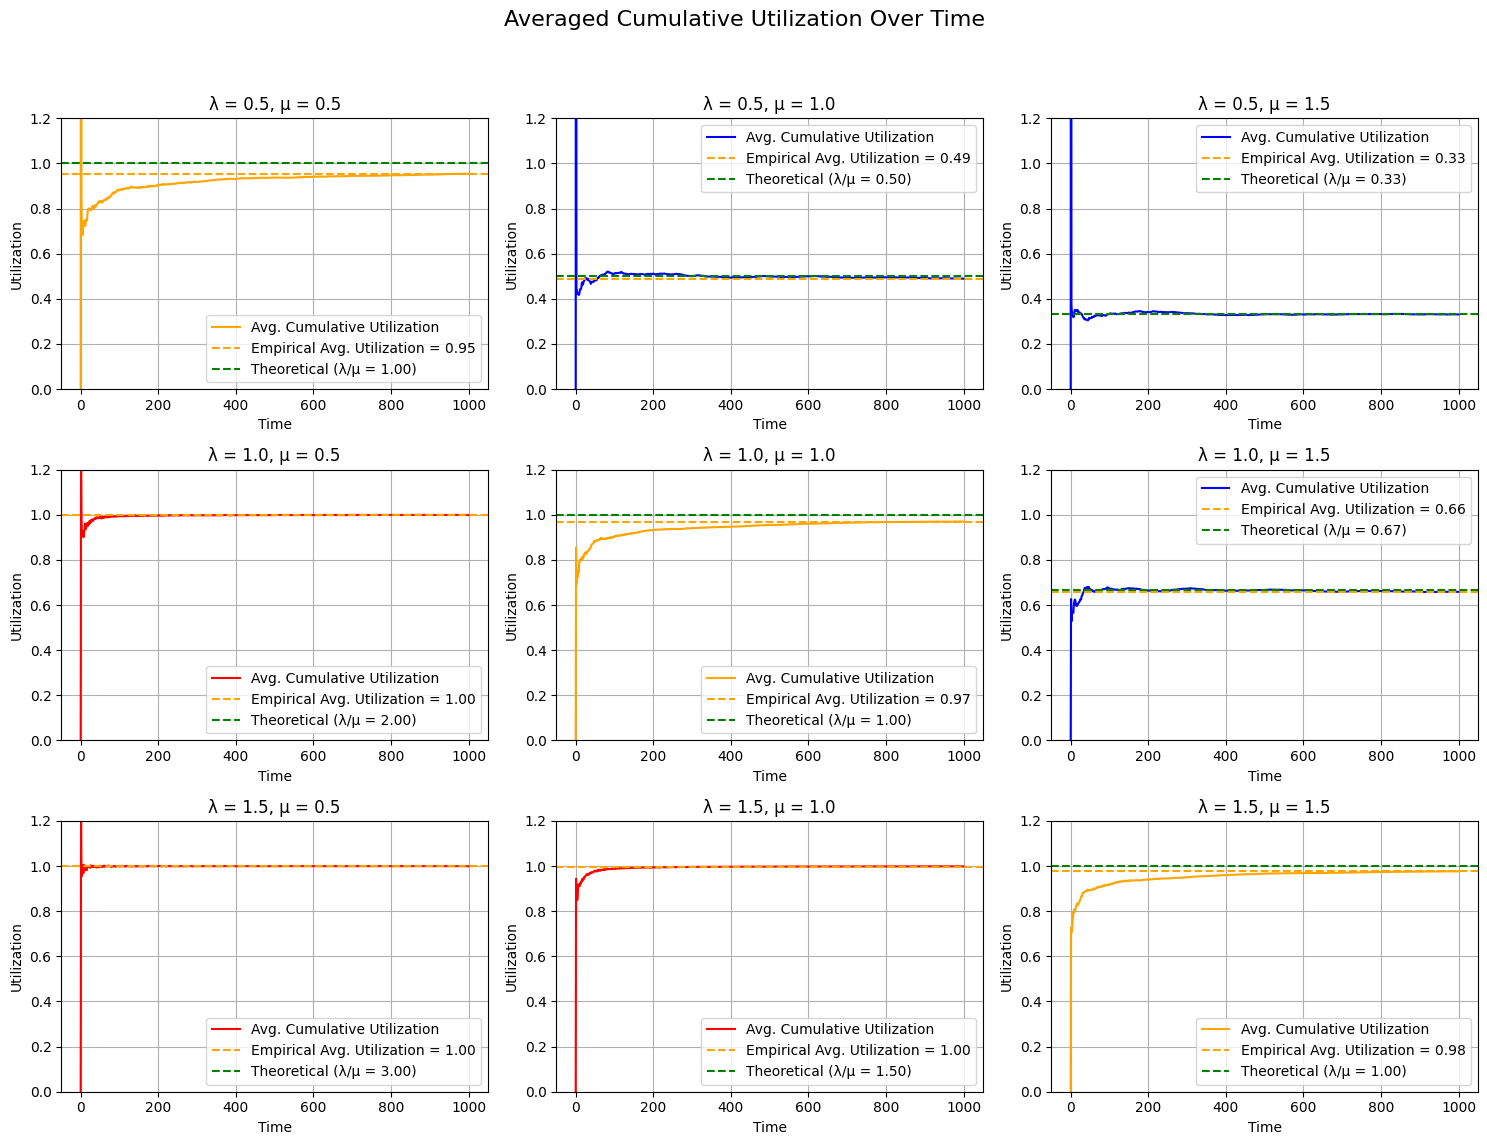
\includegraphics[width=0.8\textwidth]{images/ex1_p2_util.png}
  \caption{
    Average empirical utilization for different values of $\lambda$ and $\mu$.
    The theoretical value is shown as a dashed line.
    Red lines are the one with $\lambda > \mu$, yellow $\lambda = \mu$ and blue $\lambda < \mu$ where the system is stable.
  }\label{fig:e1p2-util}
\end{figure}

After visualizing the warming up period, we tried to estimate its length visually. We dropped the first 100 time units and computed the average utilization over the remaining 900 time units.
Figure~\ref{fig:e1p2-trunc-util} shows the truncated results, it is possible to see that the average utilization in the early period is smoother than than in previous results.

The number of truncated time units was chosen for all combinations. This was not optimal since it suits better some combinations than others.

\begin{figure}[htbp]
  \centering
  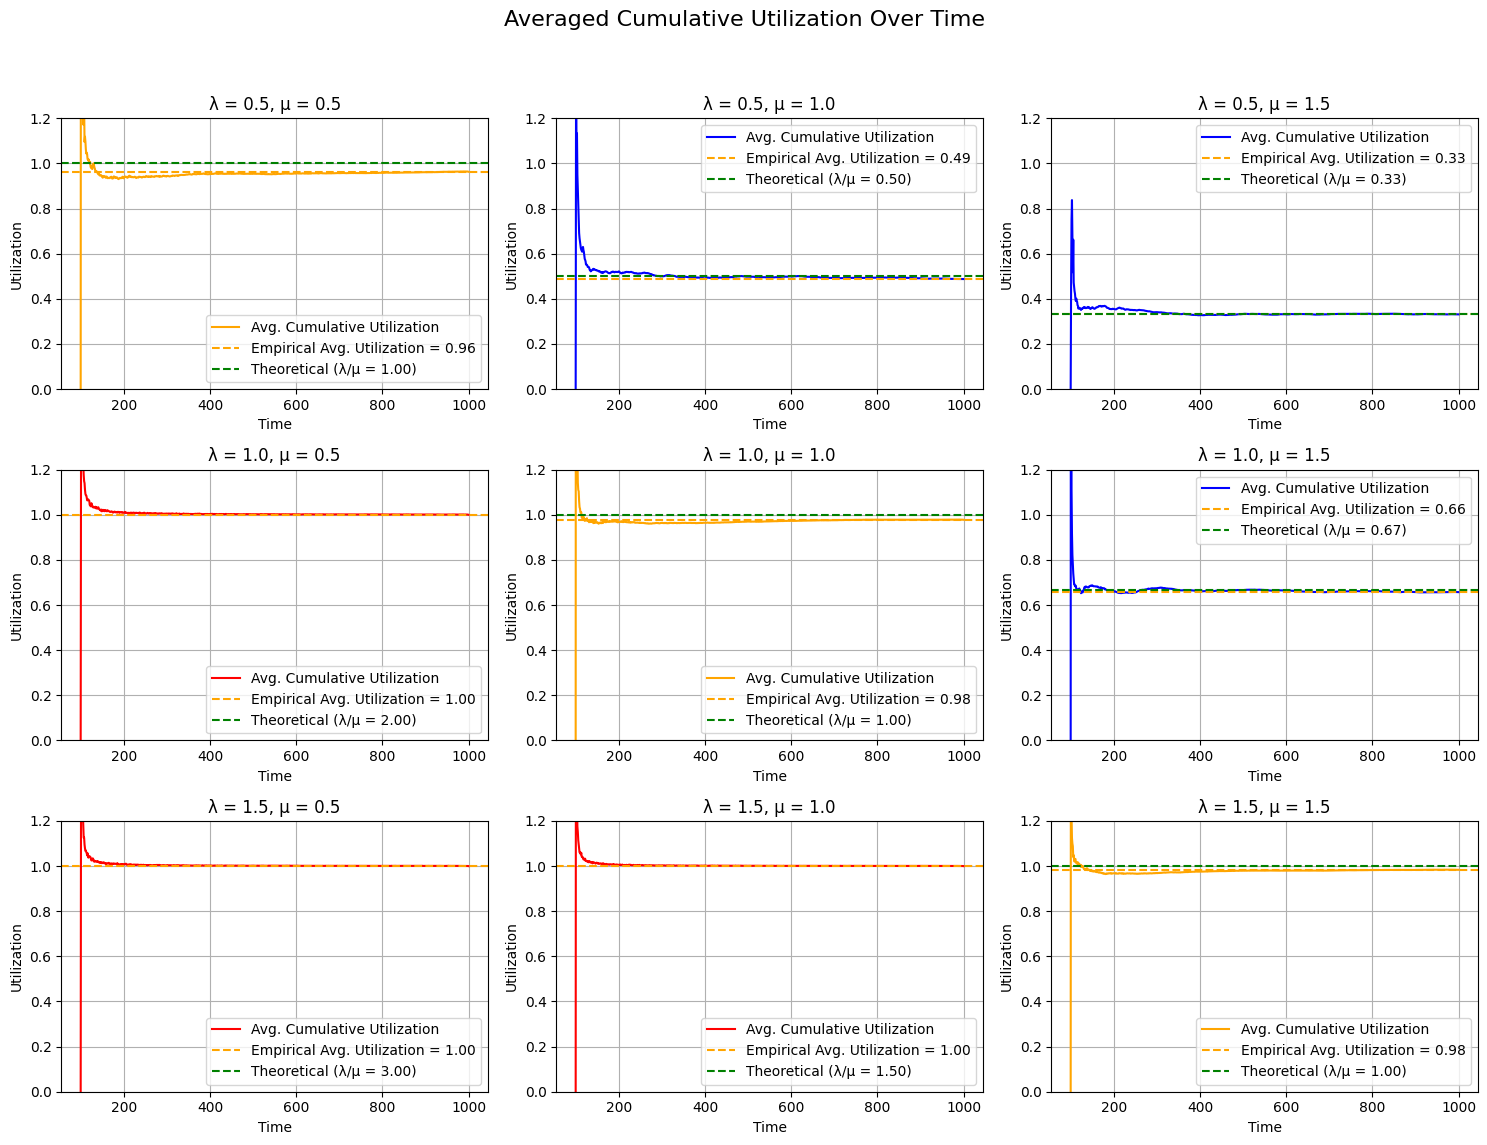
\includegraphics[width=0.8\textwidth]{images/ex1_p2_trunc_util.png}
  \caption{
    Truncated average empirical utilization for different values of $\lambda$ and $\mu$.
  }\label{fig:e1p2-trunc-util}
\end{figure}

In Figure~\ref{fig:e1p2-compare} we compare the average utilization before and after truncation only for the stable settings ($\lambda < \mu$). It shows a very small difference between the two, even a slight degradation for $\lambda = 1.0$ and $\mu = 1.5$ where higher frequency probably needed a smaller truncation period.

Also, the impact of the truncation is very small because we used independent replications that decrease the impact of the warm-up period in the first place.

\begin{figure}[htbp]
  \centering
  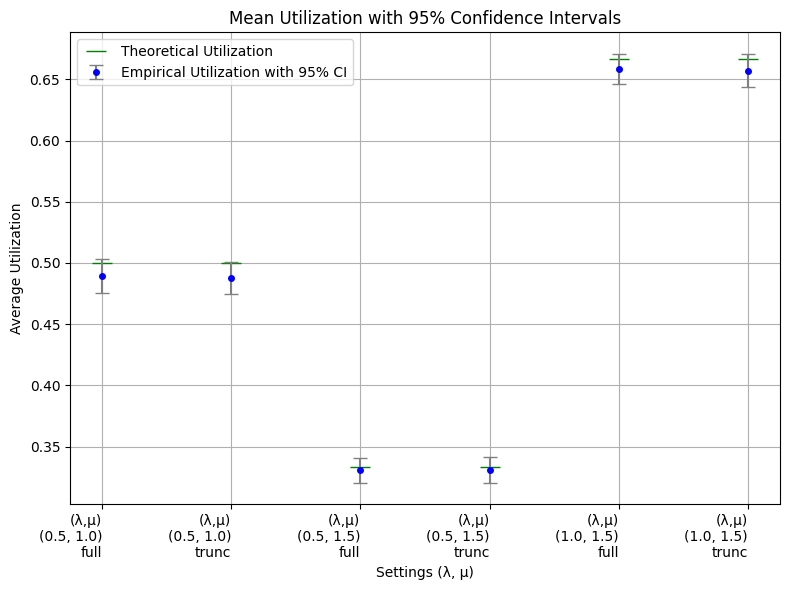
\includegraphics[width=0.8\textwidth]{images/ex1_p2_compare.png}
  \caption{
    Comparison of the average utilization before and after truncation for the stable settings ($\lambda < \mu$).
  }\label{fig:e1p2-compare}
\end{figure}

\section*{Exercise 2}

We ran a simulation with:
\begin{itemize}
    \setlength\itemsep{0.01em}
  \item $\lambda = 0.5$;
  \item $\mu = 1.5$;
  \item 100 independent replications;
  \item stopping after 10,000 time units.
\end{itemize}

With these results, we estimated the average traversal time of the packets in the system.

\subsection*{Naive estimator}

The naive estimator is simply the average of the traversal times of all packets in the system, computed as the difference between the time of arrival and the time of departure. In Figure~\ref{fig:e2p1} we show the results of the naive estimator.

\begin{figure}[htbp]
  \centering
  \begin{subfigure}[t]{0.4\textwidth}
    \centering
    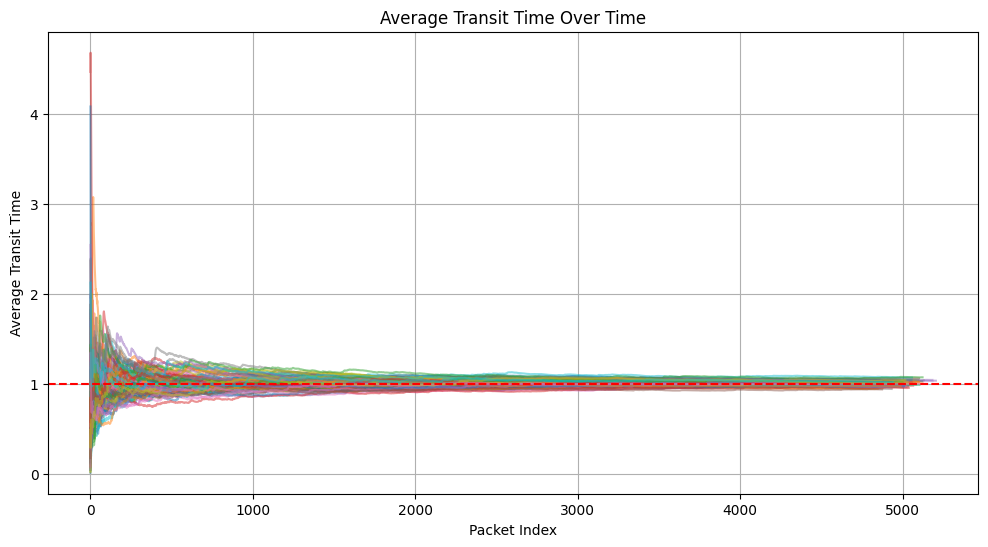
\includegraphics[width=\textwidth]{images/ex2_p1_avg_tt.png}
    \caption{
      Average traversal time over time for each replication.
    }\label{fig:e2p1-avg-tt}
  \end{subfigure}
  \hfill
  \begin{subfigure}[t]{0.4\textwidth}
    \centering
    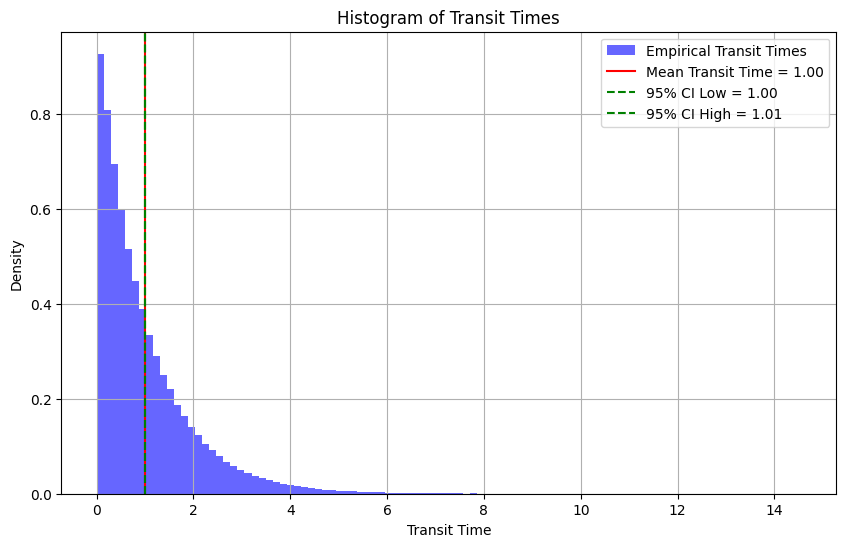
\includegraphics[width=\textwidth]{images/ex2_p1_tt.png}
    \caption{
      Histogram of all traversal times.
    }\label{fig:e2p1-tt}
  \end{subfigure}
  \caption{
    Average traversal time over time and histogram of all traversal times for the naive estimator.
  }\label{fig:e2p1}
\end{figure}

\subsection*{Using queue length as control variate}

We used the average queue length as control variate to decrease the variance of the estimator. The average queue length is computed as the weighted average of the queue length at each event, where the weight is the time elapsed since the last event.

We computed the linear regression between the average traversal time $T$ and the average queue length
$L$ form each replication, obtaining the following model:
\begin{equation}
  T = a + b \cdot L + e
\end{equation}

where $a$ is the intercept, $b$ is the slope and $e$ is the error term.

Then we the average traversal time estimator is computed as:
\begin{equation}
  \hat{T} = T - b (
    L - \mu_L
  )
\end{equation}

where $\mu_L = \frac{\rho^2}{1 - \rho}$ is the theoretical average queue length.

Figure~\ref{fig:e2p2-corr} shows the average traversal time and the average queue length for each replication. It is possible to see how the control variate removes the correlation between the two variables, making the average traversal time more stable across replications.

\begin{figure}[htbp]
  \centering
  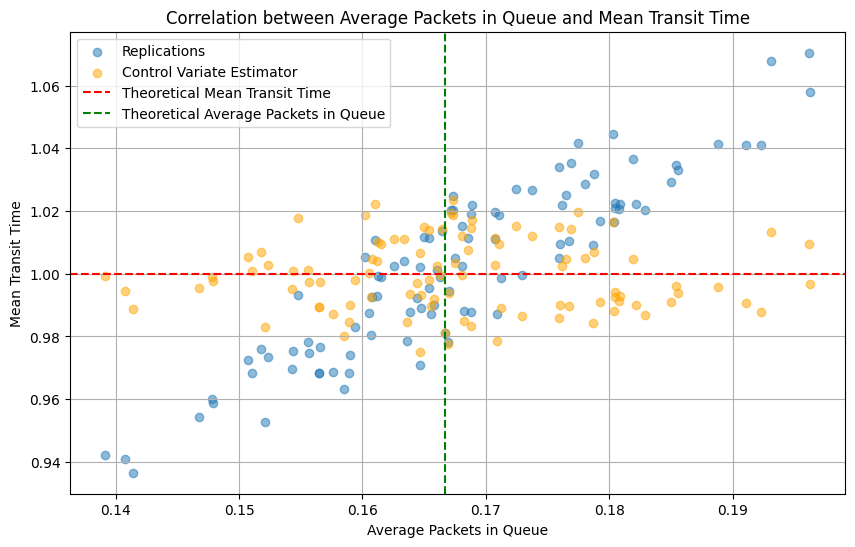
\includegraphics[width=0.8\textwidth]{images/ex2_p2_corr.png}
  \caption{
    In blue points are the average traversal time and the average queue length for each replication.
    The orange points are the average traversal time after applying the control variate.
  }\label{fig:e2p2-corr}
\end{figure}

\subsection*{Using post-stratication over packets in the system at the time of arrival}

The last estimator we implemented is based on post-stratification, where we group the traversal times by the number of packets in the system at the time of arrival (strata).

After stratifying the packets, we compute the average traversal time for each stratum and the corresponding probability of being in that stratum: $\rho^k \cdot (1 - \rho)$, where $k$ is the number of packets in the system.
Then we compute the weighted average of the traversal times, where the weights are the probabilities of being in each stratum. We must also take into account the tail of the distribution, so for the last stratum $k_{\text{max}}$ we use the probability of being in that stratum or higher, which is:

\begin{equation}
  P(X \geq k_{\text{max}}) =
  \sum_{k=k_{\text{max}}}^{\infty} P(X = k) =
  \sum_{k=k_{\text{max}}}^{\infty} \rho^k (1 - \rho) =
  \rho^{k_{\text{max}}} (1 - \rho) \cdot \sum_{k=0}^{\infty} \rho^k =
  \rho^{k_{\text{max}}} (1 - \rho) \cdot \frac{1}{1 - \rho} =
  \rho^{k_{\text{max}}}
\end{equation}

% \begin{equation}
%   \sum_{k=k_{\text{max}}}^{\infty} \rho^k (1 - \rho) =
%   (1 - \rho) \cdot \sum_{k=k_{\text{max}}}^{\infty} \rho^k =
%   \rho^{k_{\text{max}}} (1 - \rho) \cdot \sum_{k=0}^{\infty} \rho^k =
%   \rho^{k_{\text{max}}} (1 - \rho) \cdot \frac{1}{1 - \rho} =
%   \rho^{k_{\text{max}}}
% \end{equation}

\subsection*{Results}

In Figure~\ref{fig:e2p4} we show the results of the three estimators. We immediately notice the variance reduction of the in the histogram of the average traversal times (Figure~\ref{fig:e2p4-dist}).
The naive estimator is obviously the worst one, with a very high variance in comparison to the other two.
The control variate estimator (Figure~\ref{fig:e2p4-res}) has a lower variance than the post-stratification estimator, but the latter provides a more precise estimate.

\begin{figure}[htbp]
  \centering
  \begin{subfigure}[t]{0.8\textwidth}
    \centering
    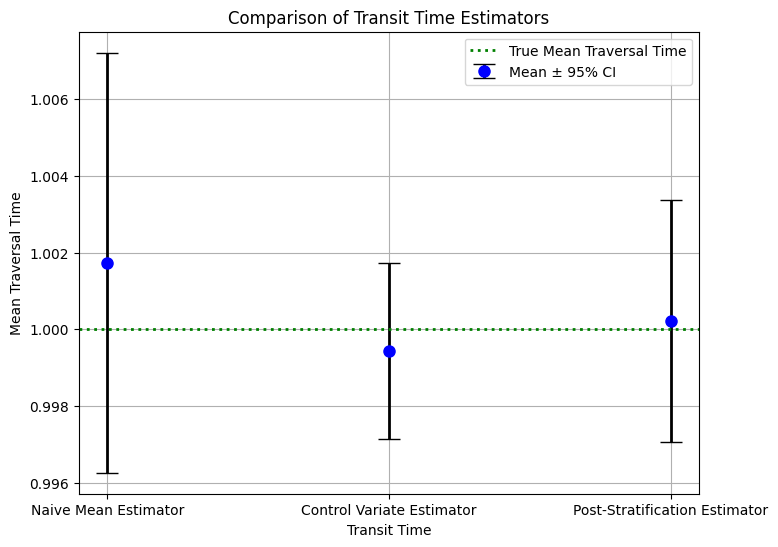
\includegraphics[width=\textwidth]{images/ex2_p4_res.png}
    \caption{
      Average traversal time for the different estimators and 95\% confidence intervals.
    }\label{fig:e2p4-res}
  \end{subfigure}
  \\
  \begin{subfigure}[t]{\textwidth}
    \centering
    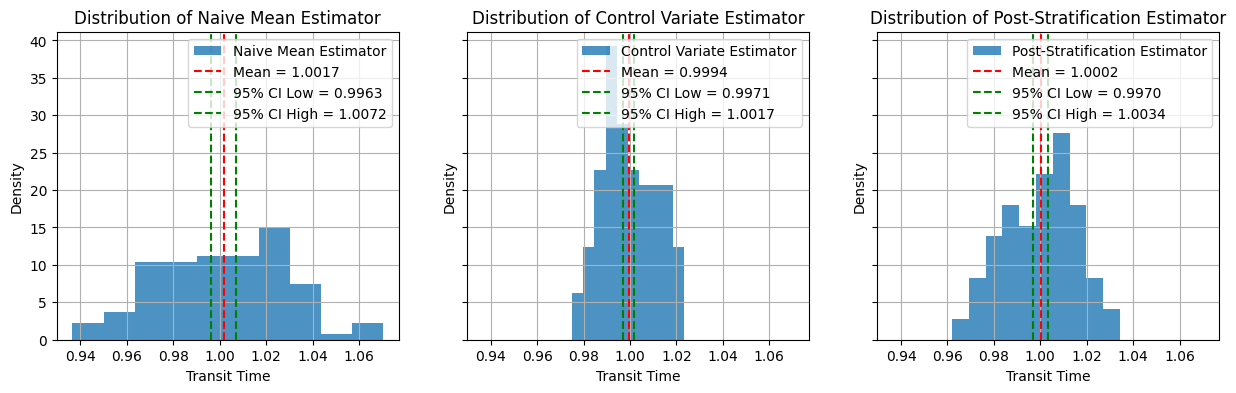
\includegraphics[width=\textwidth]{images/ex2_p4_dist.png}
    \caption{
      Histograms of the average traversal times of each replication.
    }\label{fig:e2p4-dist}
  \end{subfigure}
  \caption{
    Results of each average traversal time estimator.
  }\label{fig:e2p4}
\end{figure}

\end{document}
